Como en cada k-ésima iteración del método de la potencia estamos consiguiendo un $v^{(k)}$ autovector tentativo asociado a un $\hat{\lambda}^{(k)}$ autovalor también tentativo podemos analizar su evolución para determinar si están convergiendo y cortar la iteración cuando ya lo consideremos suficiente. Dado un $\epsilon \in \mathds{R}$ tal que $\epsilon > 0$, la matriz cuadrada $A\in \mathds{R}^{n\times n}$ sobre la cual buscamos su autovalores, y los autovalores y autovectores tentativos de la k-ésima iteración $\hat{\lambda}^{(k)} \in \mathds{R}$ y $v^{(k)} \in \mathds{R}^{n}$ planteamos los siguientes criterios de corte:

\begin{itemize}
    \item Criterio de \textit{vector residual}: cortar si $|| A v^{(k)} - v^{(k)}\hat{\lambda}^{(k)} || < \epsilon$
    \item Criterio de diferencia de autovectores: cortar si $|| v^{(k)} - v^{(k-1)} || < \epsilon$
    \item Criterio de diferencia de autovalores: cortar si $|| \hat{\lambda}^{(k)} - \hat{\lambda}^{(k-1)} || < \epsilon$
\end{itemize}

Como bajo ciertas condiciones (como $|\lambda_1| \approx |\lambda_i|$ para $\lambda_1$ autovalor dominante y $\lambda_i$ otro autovalor de la matriz $A$) el método de la potencia puede no converger, al margen de los criterios se corta la iteración tras una cantidad fija y lo suficientemente grande (de modo que si converge no interrumpa a los criterios anteriores) de veces. \\

En cuanto a precisión especulamos originalmente con que el mejor fuera el criterio de vector residual dado que mide qué tan bien aproximan $\hat{\lambda}^{(k)}$ y $v^{(k)}$ a un autovalor y autovector asociado, seguido del criterio de autovectores bajo la presunción de que funciona mejor al tener que aproximar varias componentes del autovector para terminar versus aproximar únicamente el autovalor. Bajo las mismas suposiciones especulamos livianamente que la precisión sería inversamente proporcional a la cantidad de iteraciones necesarias siendo el criterio de diferencia de autovalores el que antes se cumpliría, seguido del de autovectores y por último el de vector residual.

Sin embargo, investigando más profundamente nos encontramos con el resultado del Teorema 9.19 del libro de Burden \cite{Burden} que indica que si vale:
\begin{equation}
||A v^{(k)}-\hat{\lambda}^{(k)}v^{(k)} || < \epsilon
\end{equation}

entonces tenemos que, con $\lambda_j$ autovalores de $A$:
\begin{equation}
 \min_{j}|\lambda_j - \hat{\lambda}^{(k)}| < \epsilon
\end{equation}

Si bien da una buena idea de que el criterio de vector residual contiene en sí información sobre la convergencia de los autovalores (tentando la idea de que es más restrictivo que este criterio) no necesariamente el $\lambda_j$ más cercano a $\hat{\lambda}^{(k)}$ sea el $\lambda_1$ buscado y también podría suceder que, bajo ciertas condiciones, $\hat{\lambda}^{(k)}$ esté más cerca de $\lambda_1$ que de $\hat{\lambda}^{(k-1)}$.

El criterio de diferencia de autovectores nos resultaba interesante porque como no considera autovalores para cortar de ser lo suficientemente bueno significaría solo computarlos al final del método y no en cada iteración, además de que se condice en espiritu con el uso que le vamos a dar al resultado (solamente usar los autovectores para cambiar de base la matriz de covarianzas, sin importar los autovalores)

Otro resultado interesante en la misma sección del mismo libro es que, como indican al hablar de aceleración de convergencia, la secuencia $\{\hat{\lambda}^{(k)}\}$ converge, cuando $\lambda_1 > \lambda_2 $ con $\lambda_2$ el más grande (potencialmente no único) de los autovalores no dominantes, linealmente (más específicamente en tasa de convergencia $\mathcal{O}(\lambda_2/\lambda_1)$).
Inicialmente entendimos mal que esto significaría que la cantidad de iteraciones fuera lineal sobre $\epsilon$ sino que, por el contrario, que la tasa de convergencia sea lineal significa justamente que la sucesión se aproxima de manera lineal a $\lambda_1$ (ver definición en sección del libro \cite{Burden}), lo que implica una convergencia lenta con potencialmente muchas más iteraciones que una secuencia de convergencia, por ejemplo, cuadrática. De hecho, como se puede ver en la tabla 2.7 \cite{Burden}, una secuencia de tales características es potencialmente exponencial incluso.\\

Para experimentar usamos método de la potencia con los 3 criterios de manera separada moviendo con 20 iteraciones (sobre las que se considera promedio y desvio estandar) por valor de $\epsilon$ en un rango de $1$ a $10^{-14}$ (iteramos el exponente $i$ tal que $10^{-i}=\epsilon$ entre $0$ y $14$), el primer número resultado de una corrida en la que verificamos que el error era muy grosero como para aproximar bien autovectores y el último número resultando de probar a mano y ver que el tiempo que tardaba no lo considerábamos admisible para una ejecución cómdo (teniendo en cuenta que luego en vecinos más cercanos y PCA ibamos a iterar continuas veces el método), buscando un punto intermedio de precisión y latencia aceptables. Para medir el error usamos la inversa de la norma del mismo vector residual $|| A v^{(k)} - v^{(k)}\hat{\lambda}^{(k)} ||$. La inversa es creciente a mayor precisión y la norma del vector residual es una medida del error. De esta manera podemos usarlo como un indicador de la precision. Dado que mide 'qué tan buenos autovectores y autovalores' son los obtenidos por este método, nos resultó más atractiva que la idea de comparar contra librerias como \textit{NumPy}.

Inicialmente probamos con un set reducido de 2000 vectores (elegidos aleatoriamente sobre el total) provenientes del dataset \textit{ imdb\_small.csv} sobre los que se arma la matriz de covarianzas para poder determinar si podíamos recortar un poco más el intervalo antes de pasar al dataset entero. Consiguiendo los siguientes resultados:

\begin{figure}[h]
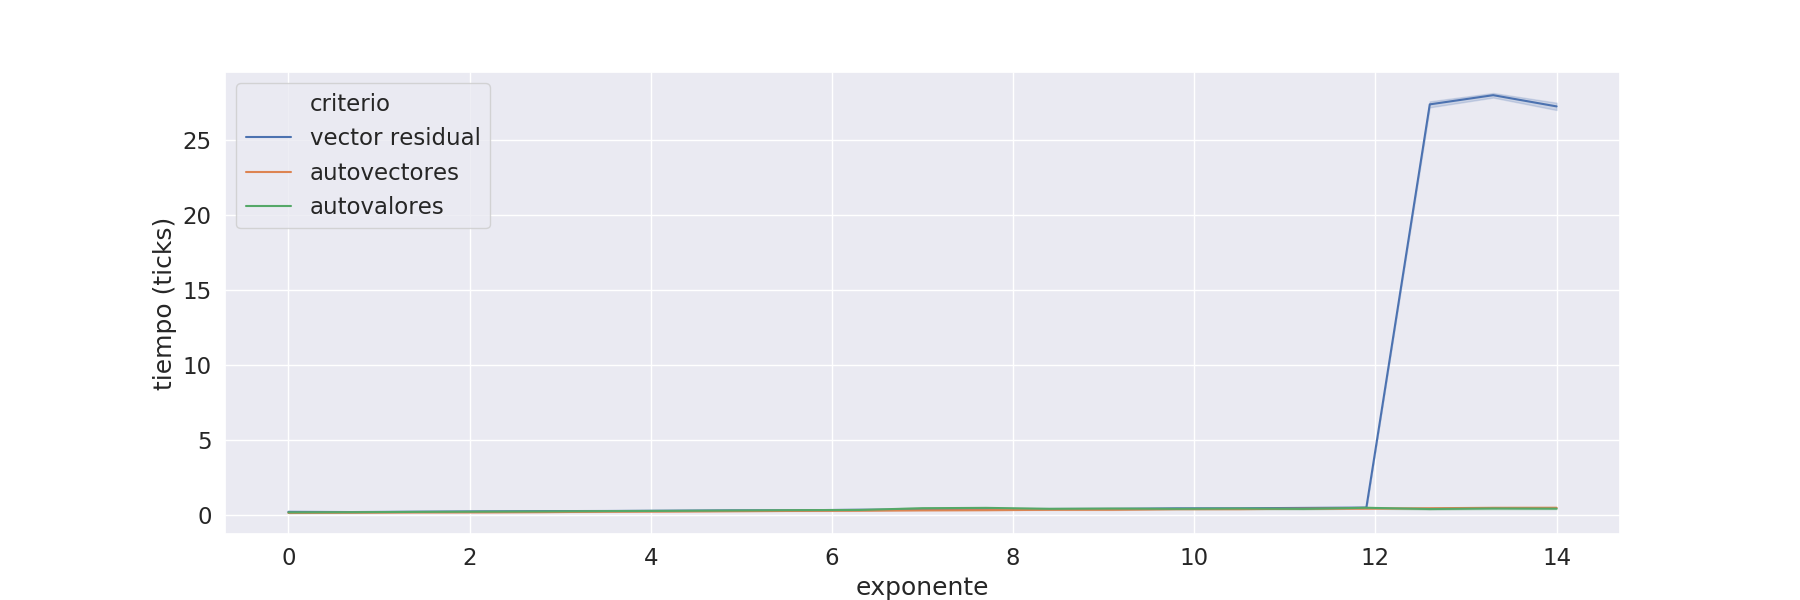
\includegraphics[width=\textwidth]{./img/tiempo_2k.png}
\centering
\caption{Progresión del tiempo medido en ticks del metodo de la potencia en función del exponente del epsilon para 2000 vectores aleatorios.\label{fig:pm_2k_t}}
\end{figure}

Como se puede ver en la figura \ref{fig:pm_2k_t} la latencia del criterio vector residual explota desmedidamente a partir del exponente $12$, como el tiempo era demasiado decidimos recortar el rango y mover el exponente solo hasta $12$ antes de pasar a medir con el dataset completo.

\begin{figure}[h]
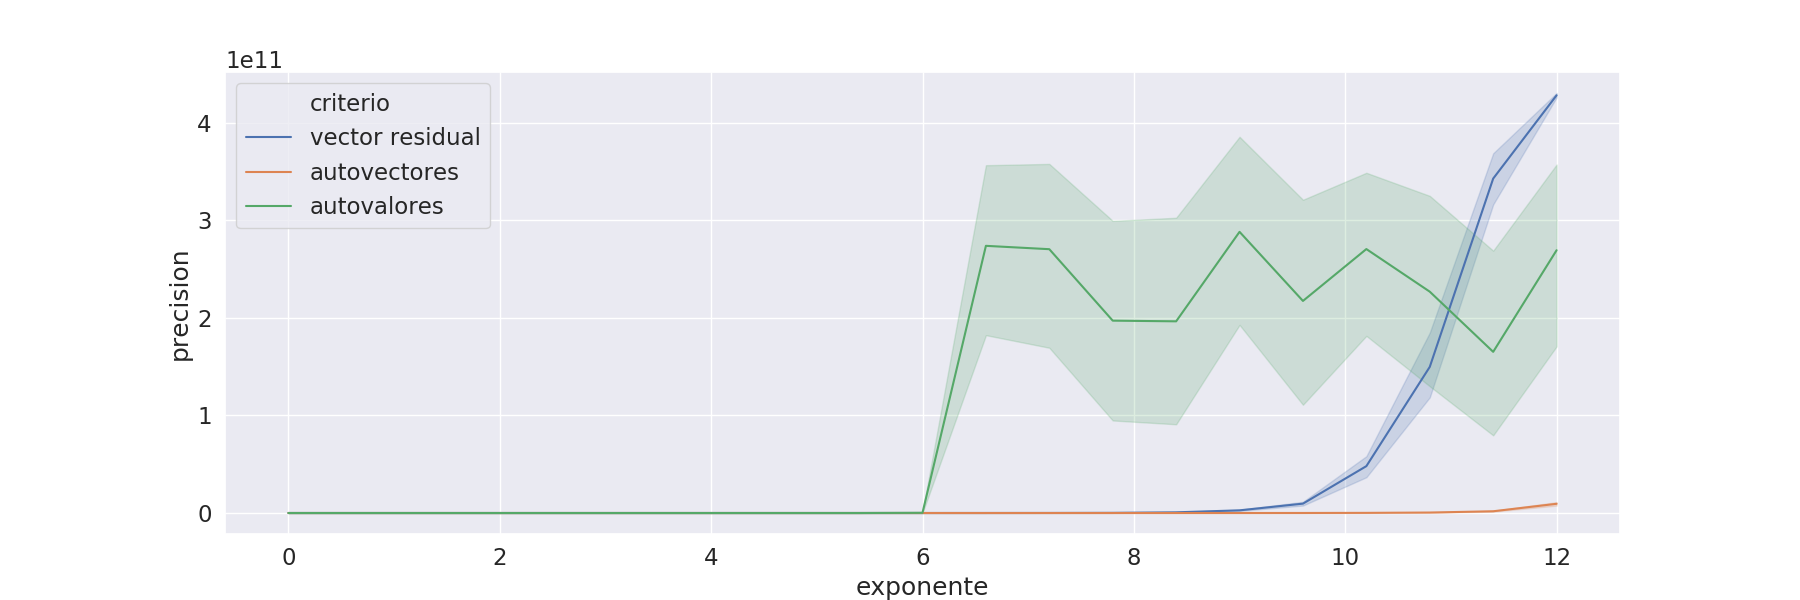
\includegraphics[width=\textwidth]{./img/precision_grande_full.png}
\centering
\caption{Progresión de precisión del metodo de la potencia en función del exponente del epsilon para los 6225 vectores del dataset.\label{fig:pm_g_p}}
\end{figure}

\begin{figure}[h]
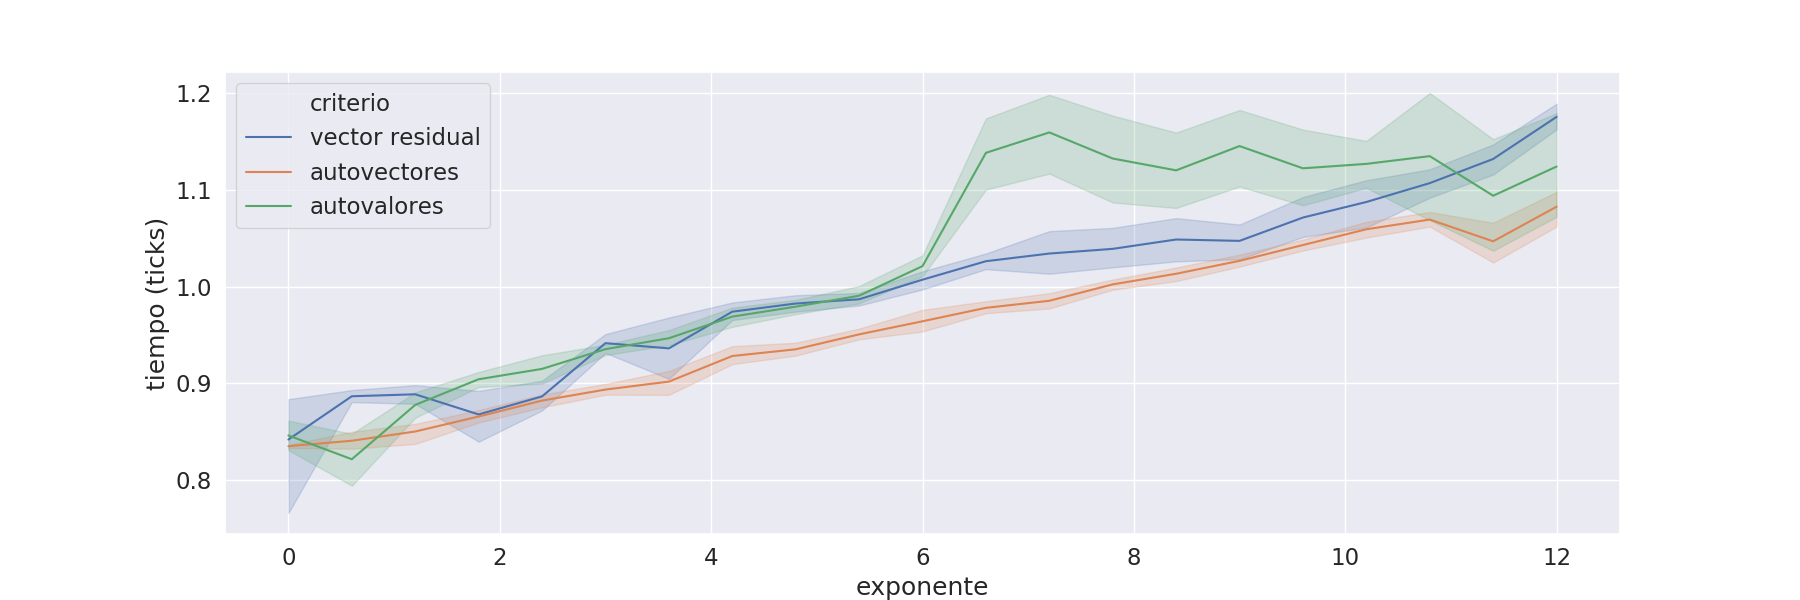
\includegraphics[width=\textwidth]{./img/tiempo_grande_full.png}
\centering
\caption{Progresión del tiempo medido en ticks del metodo de la potencia en función del exponente del epsilon para 6225 vectores del dataset.\label{fig:pm_g_t}}
\end{figure}

Vemos en la figura \ref{fig:pm_g_p} que el criterio de autovalores alcanza precisiones considerables con menos exponentes que el resto pero se mantiene inestable en variaciones y con media constante antes de que el criterio de vector residual empiece a subir de manera mucho más consistente. El criterio de autovalores recien sobre los últimos exponentes empieza a mostrar una mínima mejora.

El problema de la explosión rápida en precisión del criterio de autovalores es que viene acompañado de una explosión en latencia como indica la figura \ref{fig:pm_g_t} y en el caso del criterio de vector residual para el momento en que alcanza una precisión similar al criterio de autovalores la latencia ya es considerable (tener en cuenta que la linealidad en función del exponente significa exponencialidad respecto de epsilon para la latencia). Decidimos entonces, antes de analizar los exponentes mayores a $6$ tras la explosión del criterio de autovalores y en la subida del criterio de autovectores, analizar qué sucede antes del $6$.

\begin{figure}[h]
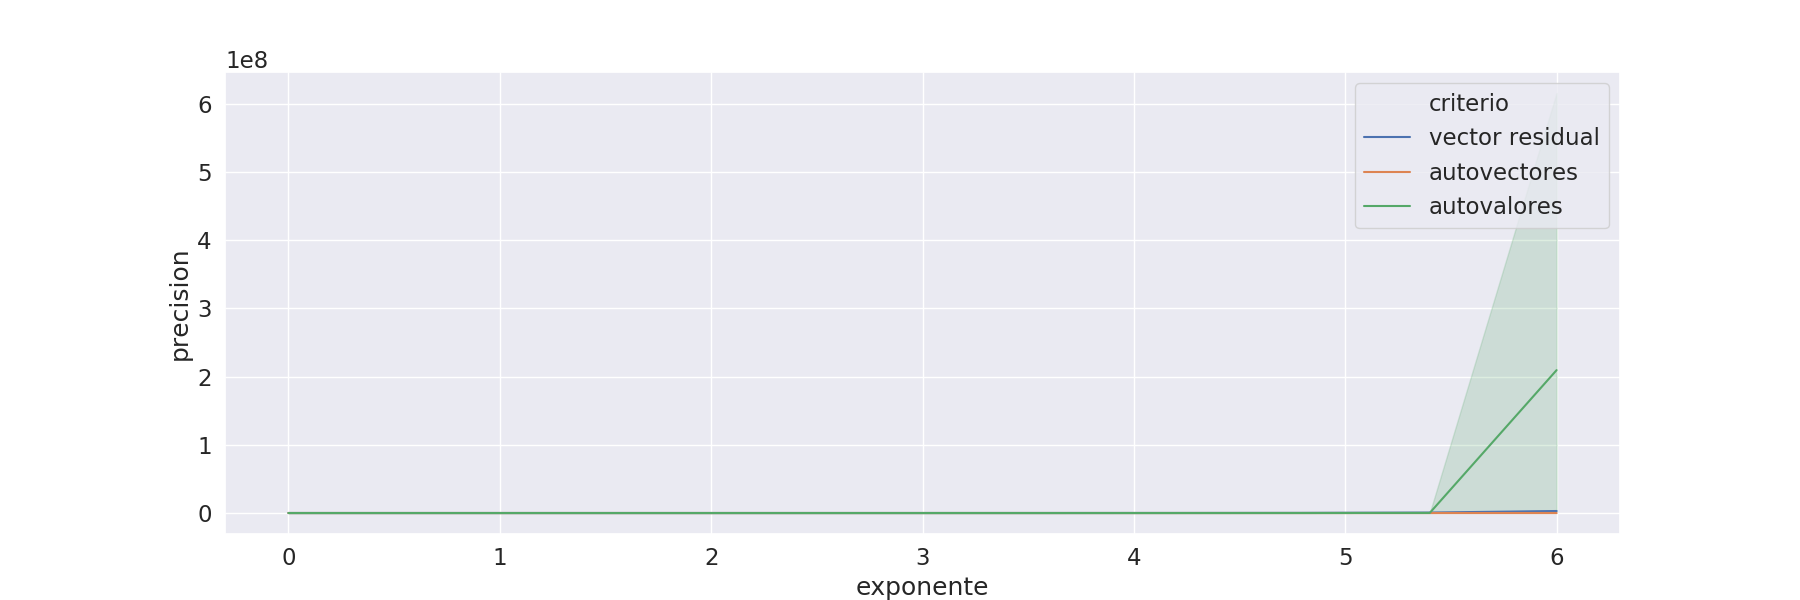
\includegraphics[width=\textwidth]{./img/precision_corto_full.png}
\centering
\caption{Progresión de precisión del metodo de la potencia en función del exponente del epsilon para los 6225 vectores del dataset. \label{fig:pm_c_p}}
\end{figure}

\begin{figure}[h]
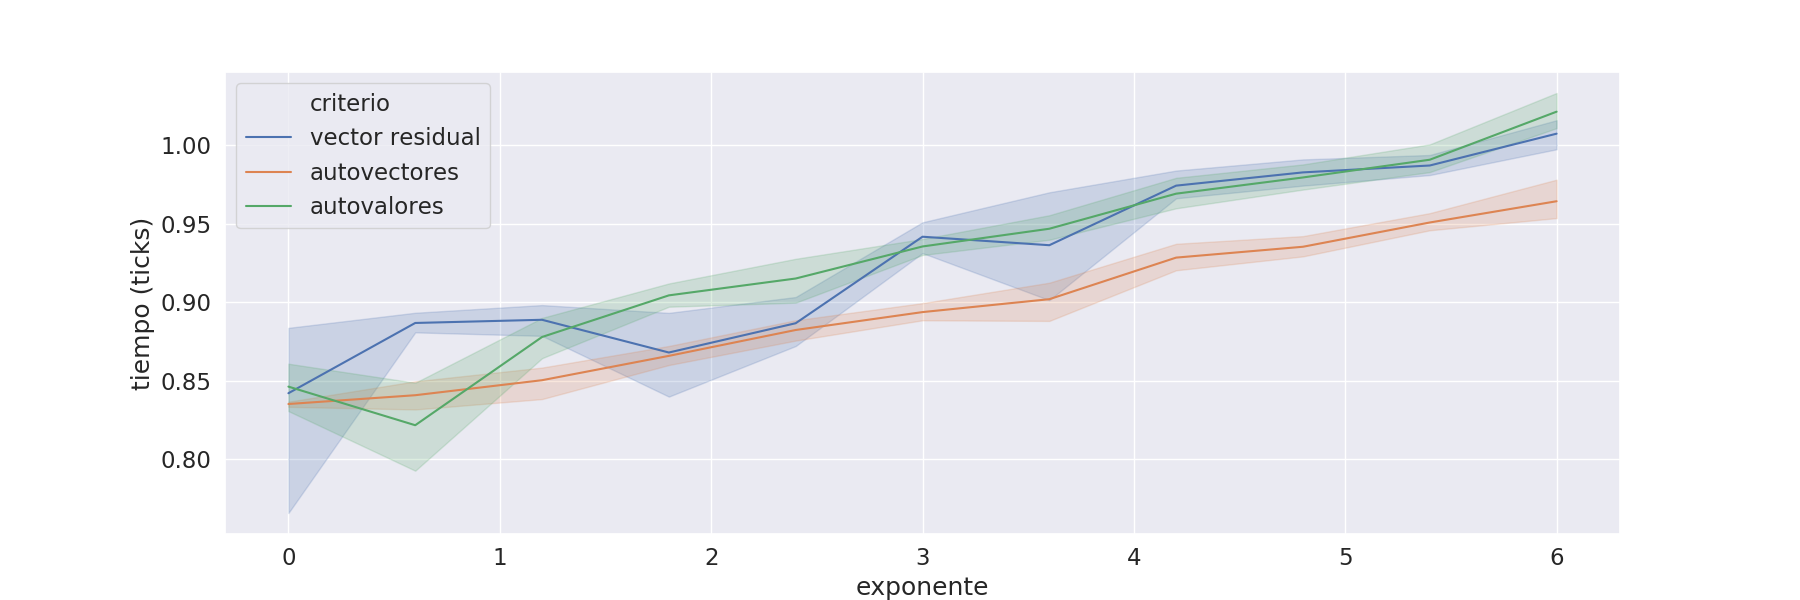
\includegraphics[width=\textwidth]{./img/tiempo_corto_full.png}
\centering
\caption{Progresión del tiempo medido en ticks del metodo de la potencia en función del exponente del epsilon para 6225 vectores del dataset. \label{fig:pm_c_t}}
\end{figure}

Viendo las figuras \ref{fig:pm_c_t} y \ref{fig:pm_c_p} consideramos que el exponente $6$ era una interesante alternativa dado que tiene en autovalores latencia mucho menor a los exponentes mayores y aun así mostraba una mejora importante de precisión respecto de exponentes menores. Decidimos entonces, antes de pasar a comparar los valores mayores a $6$ la posibilidad de comparar el criterio de autovalores para exponente $6$ contra estos (particularmente $7$, primer valor tras la explosión) en una instancia de PCA con $k$ y $\alpha$ fijos arbitrarios, dado que solamente nos interesa medir qué tan bien funcionan en un caso práctico de PCA (que es la finalidad del método) y ninguno de los dos parámetros favorece a ninguno de los dos exponentes (sí afecta $\alpha$ en cómo se arrastra errores de precisión en el método por cuestiones de deflación, pero penaliza justamente al menos preciso de modo que no nos afecta). Al iterar corridas con tales parámetros y notar que la medida de accuracy era exactamente la misma en ambos casos con tiempos favorables (cerca de la mitad en algunos casos) para el menor exponente decidimos entonces fijar $\epsilon=10^{-6}$.
